% Niveau :      PCSI
% Discipline :  Méca

\begin{exercise}{Le crayon immobile}{3}{Sup, spé}
{Mécanique,Moment cinétique,Mécanique quantique}{lelay}

On considère un crayon de papier extrêmement bien taillé, au point que sa pointe ne soit plus épaisse que d'un atome à son bout. On essaye de le poser sur la pointe de manière à ce qu'il reste vertical le plus longtemps possible. 
On appelle $\theta$ l'inclinaison du crayon par rapport à la verticale et $J$ son moment d'inertie par rapport au point où est posée la pointe, supposé immobile.

\begin{questions}
    \question Modéliser la situation, faire un schéma.
    \question \'Etablir l'équation du mouvement de du crayon lors de sa chute.
    \question On s'intéresse au mouvement initial. Réécrire l'équation précédente dans la limite des petits angles. Cette équation est-elle stable en $\theta = 0$ ?
    \question Donner une estimation numérique du temps caractéristique de chute du crayon $\tau$.
    \question Résoudre l'équation précédente pour un angle initial $\theta_0$ et un moment angulaire initial $L_0 = \frac{J}{\tau} \theta_0$. Quelle est la condition nécessaire pour que le crayon reste vertical ? Pensez-vous que ce soit (en théorie du moins) réalisable ?
    \question En réalité, la relation d'indétermination de Heinsenberg impose $\theta_0 L_0 \geq \frac{\hbar}2$. Quel est alors le $\theta_0$ minimal atteignable ?
    \question Exprimer $t_1$, le temps auquel $\theta = \theta_1$ radians, en fonction de $\tau$ et de $\theta_0$. 
    \question Le temps de chute du crayon entre $\theta_1$ et $\frac\pi2$ est $t_2 = \tau \: I(\theta_1)$ où $I$ est une fonction que l'on ne cherchera pas à exprimer. \\
    Donner le temps maximal de chute d'un crayon. Ce résultat vous semble-t-il étonnant ?
\end{questions}

\plusloin
Retrouver l'expression de la fonction $I$ sous forme d'une intégrale.

\paragraph{Donnée :}~\vspace{-3em}\\
\begin{figure}[H]
    \centering
    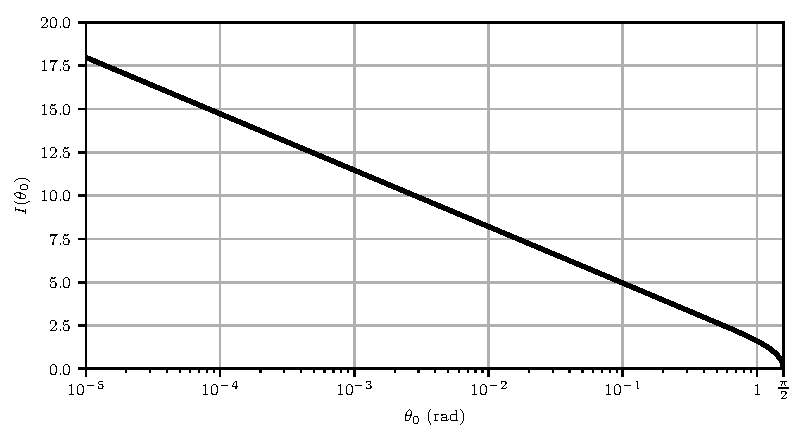
\includegraphics[scale=1]{meca/fonction_Ilog.pdf}
    \vspace{-1em}
    \caption{Graphe de la fonction $I(\theta_0)$.}
    \end{figure}
\end{exercise}